\chapter{Resultados del Algoritmo Genético}

En este capítulo presentamos los resultados obtenidos con el AG.

En la \figurename{~\ref{EjcalifMejoresHijos}} vemos las calificaciones de las mejores asignaciones.

\begin{figure}[H]
\centering
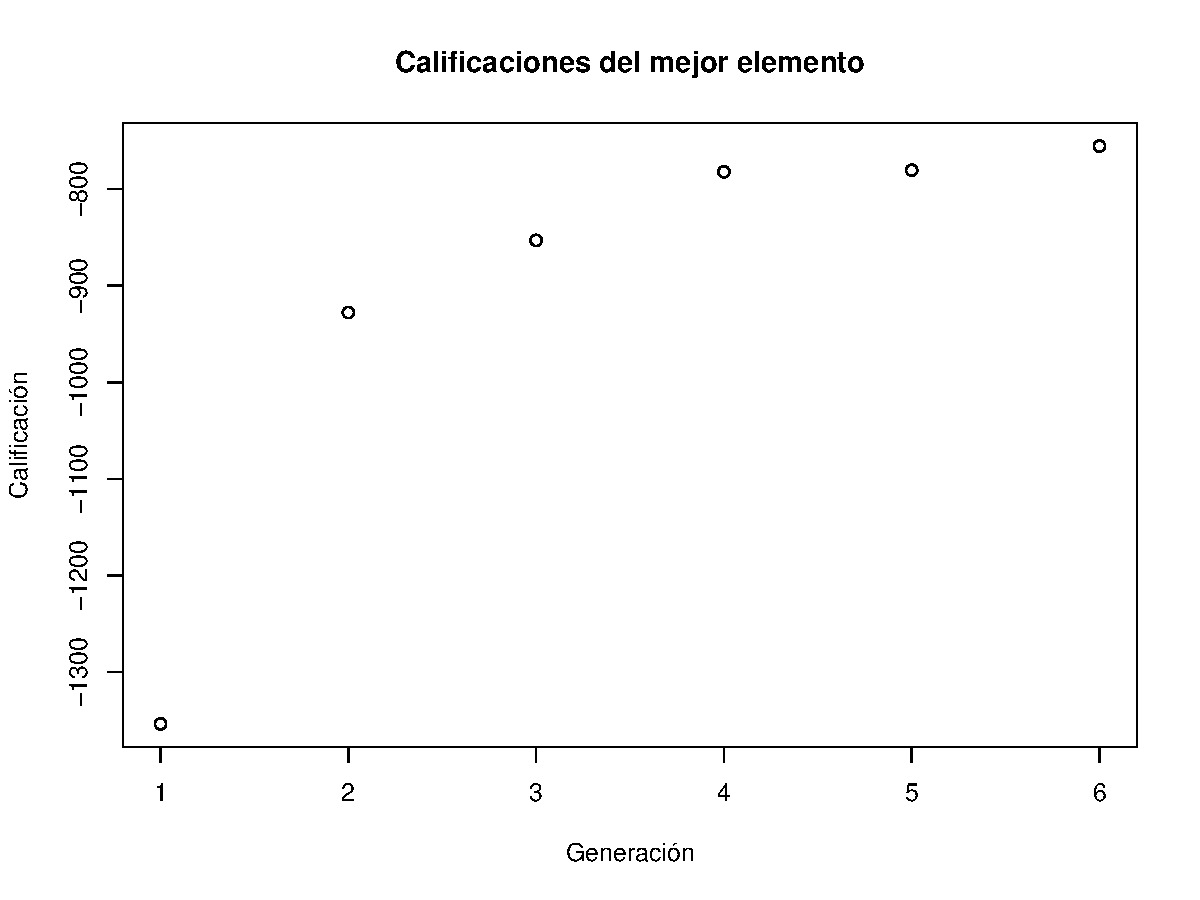
\includegraphics[width=\textwidth]{calif_mejores_hijos.pdf} %scale = 0.7
\caption{\textit{Ejemplo con calificaciones de mejores asignaciones.}}\label{EjcalifMejoresHijos}
\end{figure}

%En la \figurename{~\ref{EjcalifAsig}} vemos las calificaciones de las asignaciones.
%
%\begin{figure}[H]
%\centering
%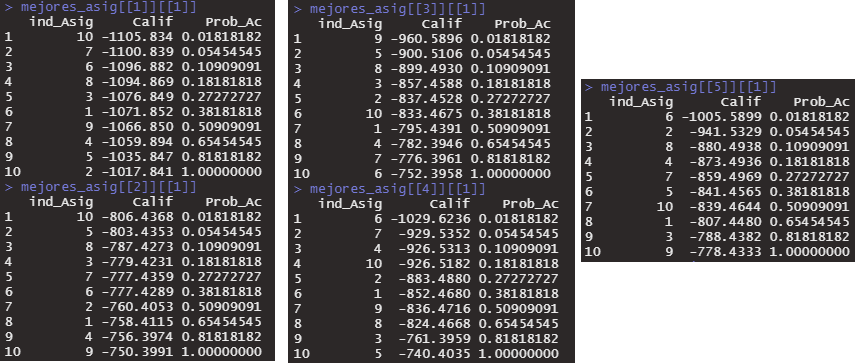
\includegraphics[width=\textwidth]{ej_calif_asignaciones} %scale = 0.7
%\caption{\textit{Ejemplo con calificaciones de asignaciones.}}\label{EjcalifAsig}
%\end{figure}

En la \figurename{~\ref{EjcalifAsig_x_generacion}} vemos las calificaciones de las asignaciones por generación. Cada línea representa una generación.

\begin{figure}[H]
\centering
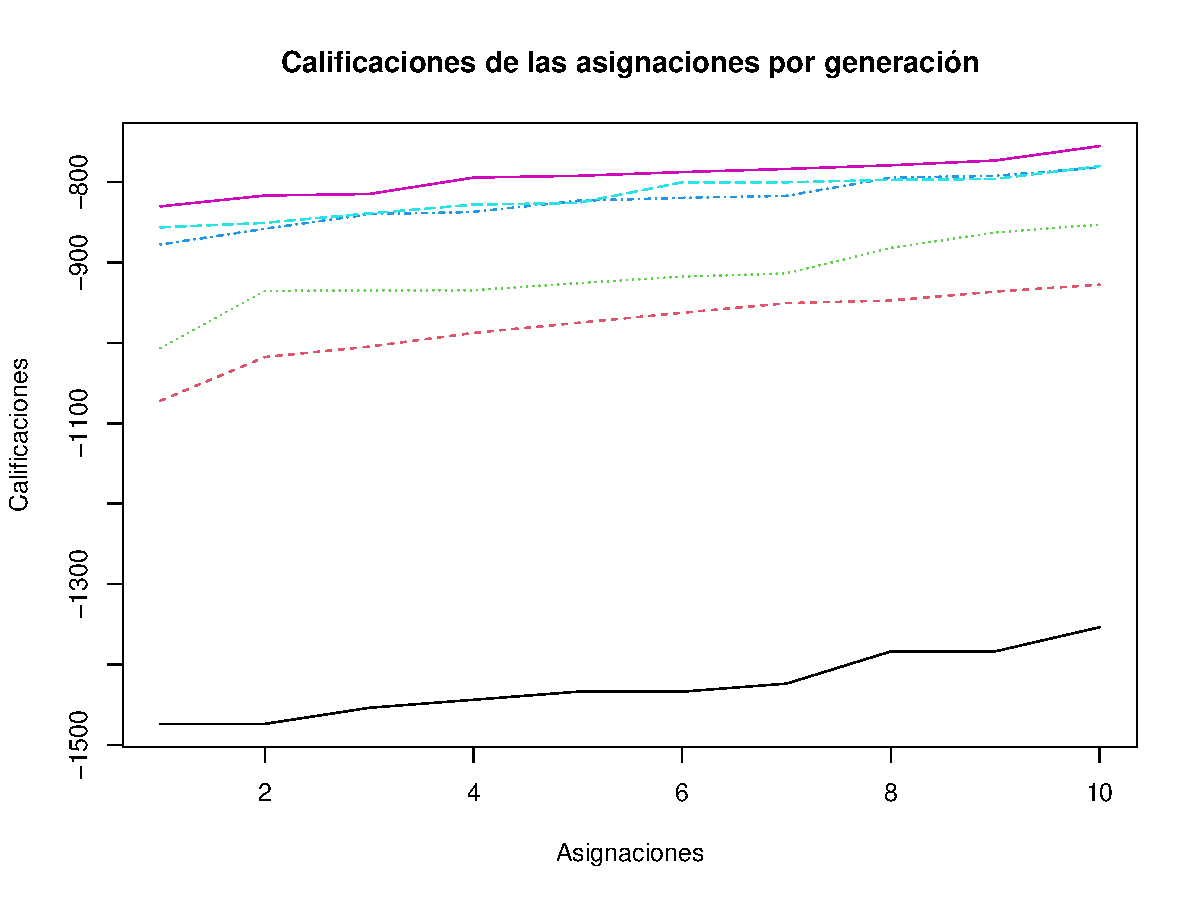
\includegraphics[width=\textwidth]{calif_asig_x_generacion.pdf} %scale = 0.7
\caption{\textit{Ejemplo con calificaciones de asignaciones por generación.}}\label{EjcalifAsig_x_generacion}
\end{figure}


Para obtener la matriz con la asignación final se simularon $g$ generaciones. El tamaño de la población es de \textit{tam\_poblacion}. Una vez terminado el proceso se extrajo el mejor elemento de la última generación. Éste elemento es la matriz que presentamos a continuación. Cabe aclarar que los datos se ordenaron con respecto a la materia (en orden alfabético) y por hora (de menor a mayor).

\dfNmatAsigFinal